
\thispagestyle{empty}


\hfill
\begin{minipage}{100mm}\begin{spacing}{1.0}

\subsection*{著者紹介}

\noindent
\begin{tabular}[t]{@{}lp{75mm}@{}}
  \multicolumn{2}{@{}l@{}}{\emph{マーチン・シェーベル(Martin Schoeberl)}}\\
  \\[-2mm]
  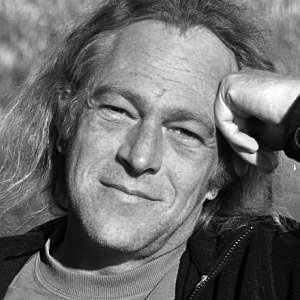
\includegraphics[height=27mm]{chisel-book-ja/Martin-BW.jpg}
  &
  \raisebox{12.5mm}{
  \begin{minipage}{68mm}\normalfont\small
  % マーチン・シェーベル\,は、
  % デンマークのコンゲンス・リュンビューにある\,%
  デンマークのリュンビューにある\,%
  デンマーク工科大学\,の\,応用数学・コンピュータサイエンス学科\,の准教授。
  研究テーマは、ハード・リアルタイム・システム、時間予測可能なコンピュータ・アーキテクチャ、リアルタイムJavaなど。
  オーストリアのウィーン工科大学でコンピュータ工学の博士号および大学教員資格を取得。
  IEEEおよびACMの会員。
  \end{minipage}
  }
  \\
\end{tabular}

\ifshoworiginal
Martin Schoeberl is an associate professor with the Department of Applied Mathematics
and Computer Science, Technical University of Denmark, Lyngby, Denmark.
His research interests include hard real-time systems, time-predictable computer architecture,
and real-time Java. He received a PhD and a Habilitation degree in computer engineering
from the Vienna University of Technology, Vienna, Austria. 
He is a member of the IEEE and the ACM.
\fi

\bigskip

\subsection*{翻訳者紹介}
\vspace{1mm}
\noindent
\emph{宗藤 誠治(むねとう せいじ)}
\\
\\[-3mm]
{\small
1992年東北大学卒業、日本アイ・ビー・エム株式会社入社。
東京基礎研究所に所属、情報セキュリティ、ソフトウェア工学、最先端半導体技術に関する研究開発に従事。
RISC-Vを使ったIoT向けのプロセッサの開発でChiselを利用。情報処理学会、IEEE および ACM の会員。博士(情報学)。
}
\\
\\[-1mm]
\noindent
\emph{七夕 雅俊(たなばた まさとし)}
\\
\\[-3mm]
{\small
2008 年武蔵工業大学(現東京都市大学)卒業、富士通LSIソリューション株式会社(現Socionext)に入社し、ネットワークアクセラレータIPの開発に従事。
その後LeapMind株式会社に入社し、AI推論アクセラレータIPの開発を担当。個人的興味からChiselの調査を行っており、その内容について各種媒体で発信。
}
\\
\\[-1mm]
\noindent
\emph{萩野 孝明(はぎの たかあき)}
\\
\\[-3mm]
{\small
電子楽器メーカ勤務。映画と音楽と車を愛し、Sequencerと縁が深い。
自作6800に始まり、TK-80, PET-8K, BUBCOM80, PC98, PC/ATと進む。
古い言語は得意だが、21世紀からVerilog/HDLを学習し自作CPU, LLVM, RISC-Vと順当に進み、Chiselへとたどり着き勉強中(いまココ)
}


\end{spacing}\end{minipage}

\clearpage

